\chapter{Acides et bases~: Ka et pKa}\label{ch:g12:ka-and-pka}

Beaucoup de fourmis se défendent avec de l'acide méthanoïque, qui brûle
la peau. L'acide méthanoïque est un petit
\omterm{def:g11:functional-groups:carboxylic-acid}{acide carboxylique}. De l'acide chlorhydrique à la même concentration
brûlerait bien davantage. Ce sont deux acides~; tous deux donnent une
solution de \omterm{def:g9:acids-bases-ph:ph}{pH} inférieur à 7~; pourtant, ils ne sont pas acides de la
même façon. Pour décrire complètement un acide, il faut deux nombres~:
la quantité présente, c'est-à-dire sa concentration, et la facilité avec
laquelle il cède son \omterm{def:g9:ions:ion}{ion} hydrogène, c'est-à-dire sa \omterm{def:g12:ka-and-pka:ka}{constante d'acidité}.

\begin{recall}
Les \omterm{def:g9:acids-bases-ph:acidic}{solutions acides}, basiques et neutres~; l'échelle de \omterm{def:g9:acids-bases-ph:ph}{pH}, de 0 à
14~: le \omterm{def:g9:acids-bases-ph:ph}{pH} est d'autant plus bas que les \omterm{def:g9:ions:ion}{ions} hydrogène sont nombreux
(\cref{ch:g9:acids-bases-ph}). Le \omterm{def:g12:equilibrium:quotient}{quotient de réaction} $Q$ et la
\omterm{def:g12:equilibrium:constant}{constante d'équilibre} $K$ (\cref{ch:g12:equilibrium}). Une \omterm{def:g12:curly-arrows:curly-arrow}{flèche courbe}
représente le déplacement d'un doublet d'\omterm{def:g9:inside-the-atom:nucleus}{électrons}
(\cref{ch:g12:curly-arrows}).
\end{recall}

\begin{omfigure}
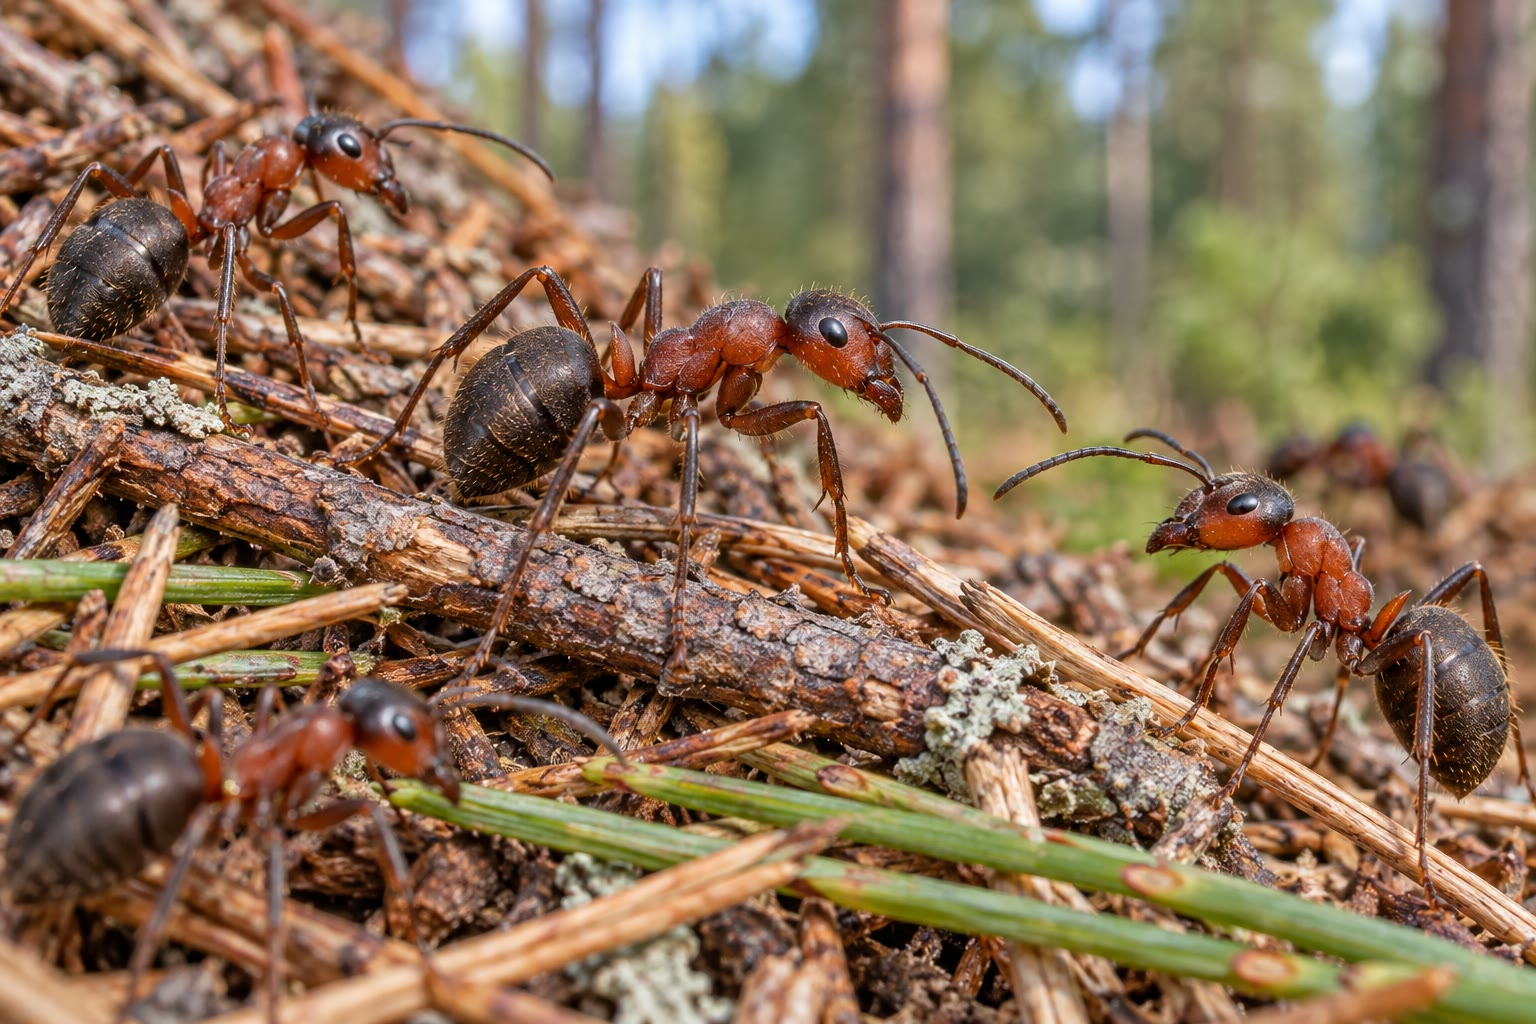
\includegraphics[width=0.45\linewidth]{images/book1/ai/g12-red-ants.jpg}

{\small Des fourmis rousses des bois~: comme beaucoup de fourmis, elles se défendent avec de l'acide méthanoïque.}
\end{omfigure}

\section{Acides et bases de Brønsted}

\begin{definition}[Acide et base de Brønsted, couple acide/base]\label{def:g12:ka-and-pka:bronsted}
Un \emph{acide de Brønsted}\index{acide de brønsted@acide de Brønsted} est une espèce
capable de céder un \omterm{def:g9:ions:ion}{ion} hydrogène \ce{H+}~; une \emph{base de
Brønsted}\index{base de brønsted@base de Brønsted} est une espèce capable d'en capter un.
Un acide HA et la base \ce{A-} qu'il devient en perdant \ce{H+} forment
un \emph{couple acide/base}\index{couple acide/base},
noté \ce{HA}/\ce{A-}~: $\ce{HA} \rightleftharpoons \ce{A-} + \ce{H+}$.
\end{definition}

\begin{definition}[Ion oxonium, ampholyte]\label{def:g12:ka-and-pka:oxonium}
Dans l'eau, un \omterm{def:g9:ions:ion}{ion} hydrogène ne reste jamais seul~: il est capté par une
\omterm{def:g7:atoms-and-molecules:molecule}{molécule} d'eau, ce qui donne l'\emph{ion oxonium}\index{ion oxonium}
\ce{H3O+}. Une espèce qui est l'acide d'un couple et la base d'un autre
est un \emph{ampholyte}\index{ampholyte}~; l'eau en est un~: acide du
couple
\ce{H2O}/\ce{OH-} et base du couple \ce{H3O+}/\ce{H2O}.
\end{definition}

\begin{example}[Un acide dans l'eau]\label{ex:g12:ka-and-pka:acid-water}
Quand l'acide éthanoïque \omterm{def:g2:mixing-and-dissolving:dissolve}{se dissout}, un \omterm{def:g10:lewis-and-shape:lone-pair}{doublet non liant} d'une \omterm{def:g7:atoms-and-molecules:molecule}{molécule}
d'eau capte l'hydrogène de sa liaison \ce{O-H}, et le doublet de
\ce{O-H} reste sur l'oxygène de l'acide~:
\[
  \ce{CH3COOH + H2O <=> CH3COO- + H3O+} .
\]
Deux couples échangent un \omterm{def:g9:ions:ion}{ion} hydrogène~: \ce{CH3COOH}/\ce{CH3COO-} le
cède,
\ce{H3O+}/\ce{H2O} le capte. Désormais, les \omterm{def:g9:ions:ion}{ions} hydrogène des chapitres
précédents s'écrivent \ce{H3O+} chaque fois que l'eau est le \omterm{def:g6:solutions-and-solubility:solute}{solvant}.
\end{example}

\begin{omfigure}
\setchemfig{atom sep=2em}
\chemfig{H_3C-C(=[2]O)-O-[@{oh}]@{h}H}\qquad
\chemfig{@{ow}\charge{90=\:,270=\:}{O}(-[:150]H)-[:210]H}
\qquad$\longrightarrow$\qquad
\chemfig{H_3C-C(=[2]O)-\charge{90=\:,0=\:,270=\:}{O}^{-}}\quad$+$\quad\ce{H3O+}
\chemmove{
  \draw[->, thick, omProp, shorten <=4pt, shorten >=3pt]
    ($(ow)+(0,0.25)$) .. controls +(110:9mm) and +(60:9mm) .. (h);
  \draw[->, thick, omDef, shorten <=2pt, shorten >=4pt]
    (oh) .. controls +(-90:7mm) and +(-60:6mm) .. ($(oh)+(-0.3,-0.2)$);}

{\small Un \omterm{def:g9:ions:ion}{ion} hydrogène passe de l'acide à l'eau~: un \omterm{def:g10:lewis-and-shape:lone-pair}{doublet non liant}
de l'eau forme la nouvelle liaison \ce{O-H} (en orange), et l'ancien
doublet \ce{O-H} reste sur l'oxygène de l'\omterm{def:g9:ions:ion}{ion} éthanoate (en bleu).}
\end{omfigure}

\begin{history}[D'Arrhenius à Brønsted, 1887--1923]
En 1887, Svante Arrhenius proposa que les acides libèrent des \omterm{def:g9:ions:ion}{ions}
hydrogène dans l'eau, et les bases des \omterm{def:g9:ions:ion}{ions} hydroxyde. En 1923, Johannes
Brønsted et, indépendamment, Thomas Lowry élargirent cette idée~: un
acide est toute espèce qui cède un \omterm{def:g9:ions:ion}{ion} hydrogène, une base toute espèce
qui en capte un, dans l'eau ou non. La \omterm{def:g7:atoms-and-molecules:molecule}{molécule} d'ammoniac, qui ne
contient pas d'hydroxyde, devint une base comme les autres.
\end{history}

\begin{omfigure}
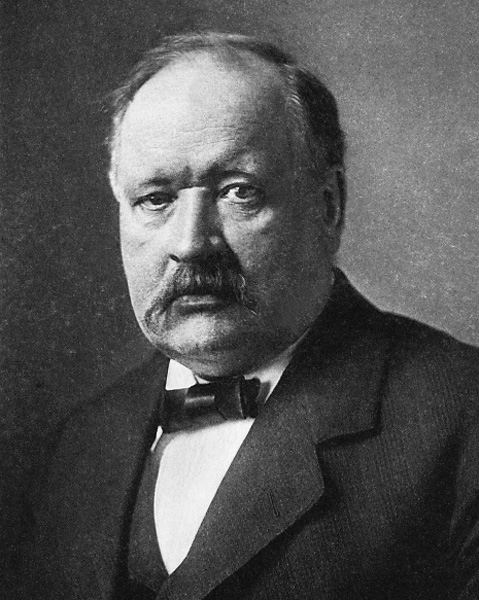
\includegraphics[width=0.22\linewidth]{images/book1/arrhenius.jpg}

{\small Svante Arrhenius (1859--1927).}
\end{omfigure}

\section{Le pH, de façon quantitative}

\begin{definition}[Le pH, précisément]\label{def:g12:ka-and-pka:ph-log}
Dans une \omterm{def:g6:solutions-and-solubility:solute}{solution aqueuse} diluée, le \omterm{def:g9:acids-bases-ph:ph}{pH} est défini par
\[
  \mathrm{pH} = -\log\frac{[\ce{H3O+}]}{c^\circ},
  \qquad\text{c'est-à-dire}\qquad
  [\ce{H3O+}] = c^\circ \times 10^{-\mathrm{pH}} ,
\]
où $\log$ est le logarithme décimal.
\end{definition}

\begin{proposition}[Diluer dix fois, c'est une unité]\label{prop:g12:ka-and-pka:dilution}
Si $[\ce{H3O+}]$ est divisée par 10, le \omterm{def:g9:acids-bases-ph:ph}{pH} augmente de 1~; si elle est
multipliée par 10, le \omterm{def:g9:acids-bases-ph:ph}{pH} diminue de 1.
\end{proposition}

\begin{proof}
$-\log\big([\ce{H3O+}]/10c^\circ\big) = -\log\big([\ce{H3O+}]/c^\circ\big)
+ \log 10 = \mathrm{pH} + 1$.
\end{proof}

\begin{definition}[Acides et bases forts et faibles]\label{def:g12:ka-and-pka:strong-acid}
Un \emph{acide fort}\index{acide fort} réagit totalement avec l'eau~:
il ne reste pas d'acide sous sa forme initiale dans la solution. Un
\emph{acide faible}\index{acide faible} réagit partiellement~: sa
réaction avec l'eau aboutit à un équilibre. De même, une \emph{base
forte}\index{base forte} réagit totalement avec l'eau, une \emph{base
faible}\index{base faible} partiellement.
\end{definition}

\begin{proposition}[pH d'un acide fort]\label{prop:g12:ka-and-pka:strong}
Une solution d'\omterm{def:g12:ka-and-pka:strong-acid}{acide fort} de concentration $c$ (pas trop diluée) a
$[\ce{H3O+}] = c$ et $\mathrm{pH} = -\log(c/c^\circ)$.
\end{proposition}

\begin{proof}
La réaction \ce{HA + H2O -> A- + H3O+} est totale~: chaque \omterm{def:g7:atoms-and-molecules:molecule}{molécule}
d'acide donne un \omterm{def:g12:ka-and-pka:oxonium}{ion oxonium}. Les \omterm{def:g9:ions:ion}{ions} provenant de l'eau elle-même sont
négligeables tant que $c$ est très supérieure à \qty{e-7}{mol/L}.
\end{proof}

\begin{example}[L'acide chlorhydrique]\label{ex:g12:ka-and-pka:hcl}
Acide chlorhydrique à \qty{0.010}{mol/L}~: $[\ce{H3O+}] = \qty{0.010}{mol/L}$
et $\mathrm{pH} = -\log 0.010 = 2.0$. Dilué dix fois~: \omterm{def:g9:acids-bases-ph:ph}{pH} 3.0.
\end{example}

\section{L'eau et son produit ionique}


\begin{definition}[Produit ionique de l'eau]\label{def:g12:ka-and-pka:ionic-product}
L'eau réagit très légèrement sur elle-même, \ce{2H2O <=> H3O+ + OH-}. La
\omterm{def:g12:equilibrium:constant}{constante d'équilibre} de cette réaction est le \emph{produit ionique de
l'eau}\index{produit ionique de l'eau}~:
\[
  K_e = \frac{[\ce{H3O+}]\,[\ce{OH-}]}{(c^\circ)^2},
  \qquad pK_e = -\log K_e .
\]
\end{definition}

\begin{proposition}[L'eau neutre et les bases fortes]\label{prop:g12:ka-and-pka:ke}
% ledger: ke:25C
À \qty{25}{\celsius}, $K_e = \num{1.0e-14}$ et $pK_e = 14.0$. Dans l'eau
pure,
$[\ce{H3O+}] = [\ce{OH-}] = \qty{1.0e-7}{mol/L}$~: \omterm{def:g9:acids-bases-ph:ph}{pH} 7.0. Une \omterm{def:g12:ka-and-pka:strong-acid}{base forte}
de concentration $c$ donne $[\ce{OH-}] = c$, donc
$[\ce{H3O+}] = K_e (c^\circ)^2 / c$ et $\mathrm{pH} = 14.0 + \log(c/c^\circ)$.
\end{proposition}

\begin{proof}
Dans l'eau pure, les deux \omterm{def:g9:ions:ion}{ions} se forment par paires~: ils sont donc en
quantités égales, et leur produit vaut $\num{1.0e-14}$~: chacun vaut
\qty{1.0e-7}{mol/L}. Pour la base, $K_e$ reste vérifié dans la
solution~:
$-\log([\ce{H3O+}]/c^\circ) = -\log K_e + \log(c/c^\circ)$.
\end{proof}

\begin{example}[L'hydroxyde de sodium]\label{ex:g12:ka-and-pka:naoh}
Hydroxyde de sodium à \qty{0.010}{mol/L}~: $[\ce{OH-}] = 0.010$, donc
$[\ce{H3O+}] = \num{1.0e-14}/0.010 = \qty{1.0e-12}{mol/L}$ et \omterm{def:g9:acids-bases-ph:ph}{pH} 12.0.
\end{example}

\section{La constante d'acidité}

\begin{definition}[Constante d'acidité, $pK_a$]\label{def:g12:ka-and-pka:ka}
La \emph{constante d'acidité}\index{constante d'acidite@constante d'acidité} $K_a$ d'un
couple \ce{HA}/\ce{A-} est la \omterm{def:g12:equilibrium:constant}{constante d'équilibre} de la réaction de
l'acide avec l'eau, \ce{HA + H2O <=> A- + H3O+}~:
\[
  K_a = \frac{[\ce{A-}]\,[\ce{H3O+}]}{[\ce{HA}]\,c^\circ} .
\]
Le \emph{pKa}\index{pKa} du couple est
$pK_a = -\log K_a$.
\end{definition}

\begin{proposition}[Plus le $pK_a$ est petit, plus l'acide est fort]\label{prop:g12:ka-and-pka:compare}
De deux \omterm{def:g12:ka-and-pka:strong-acid}{acides faibles} de même concentration, celui qui a la plus grande
constante
$K_a$, c'est-à-dire le plus petit $pK_a$, réagit davantage avec l'eau et
donne le \omterm{def:g9:acids-bases-ph:ph}{pH} le plus bas~; sa base conjuguée est la plus faible.
\end{proposition}

\begin{proof}
Un $K_a$ plus grand signifie davantage de \ce{A-} et de \ce{H3O+} à
l'équilibre pour la même quantité de \ce{HA}. La base \ce{A-} d'un
couple qui cède facilement son \omterm{def:g9:ions:ion}{ion} hydrogène le reprend difficilement.
\end{proof}

\begin{omfigure}
\begin{tikzpicture}[font=\small, y=0.55cm]
  % ledger: pka:methanoic, pka:ethanoic, pka:benzoic, pka:ascorbic1, ka:HF, ka:H2CO3, ka:HCO3, kb:NH3, ke:25C
  \draw[->, thick] (0,0) -- (0,14.8) node[above] {$pK_a$};
  \foreach \k in {0,2,4,6,8,10,12,14} \draw (-0.1,\k) -- (0.1,\k) node[right, font=\scriptsize] {\k};
  \node[font=\footnotesize\bfseries, anchor=south] at (-3.0,14.3) {acide};
  \node[font=\footnotesize\bfseries, anchor=south] at (3.0,14.3) {base};
  \foreach \p/\yl/\acid/\base in {3.19/2.9/{\ce{HF}}/{\ce{F-}},
      3.74/3.6/{\ce{HCOOH}}/{\ce{HCOO-}}, 4.04/4.3/{acide ascorbique}/{ascorbate},
      4.20/5.0/{\ce{C6H5COOH}}/{\ce{C6H5COO-}}, 4.76/5.7/{\ce{CH3COOH}}/{\ce{CH3COO-}},
      6.37/6.9/{\ce{CO2,H2O}}/{\ce{HCO3-}}, 9.26/9.26/{\ce{NH4+}}/{\ce{NH3}},
      10.33/10.4/{\ce{HCO3-}}/{\ce{CO3^{2-}}}} {
    \draw[omDef] (-0.25,\p) -- (0.25,\p);
    \draw[black!40] (-0.25,\p) -- (-1.1,\yl);
    \draw[black!40] (0.25,\p) -- (1.1,\yl);
    \node[anchor=east, font=\scriptsize] at (-1.15,\yl) {\acid};
    \node[anchor=west, font=\scriptsize] at (1.15,\yl) {\base};
  }
  \draw[->, omThm, thick] (-4.6,13) -- (-4.6,1);
  \node[omThm, rotate=90, font=\footnotesize] at (-4.95,7) {acides plus forts};
  \draw[->, omMeth, thick] (4.6,1) -- (4.6,13);
  \node[omMeth, rotate=90, font=\footnotesize] at (4.95,7) {bases plus fortes};
\end{tikzpicture}

{\small Quelques couples placés selon leur $pK_a$ à \qty{25}{\celsius},
les acides à gauche, leurs bases à droite. Plus un couple est bas sur
l'échelle, plus son acide est fort~; plus il est haut, plus sa base est
forte.}
\end{omfigure}


\begin{method}[pH d'un acide faible]\label{met:g12:ka-and-pka:weak}
Pour un \omterm{def:g12:ka-and-pka:strong-acid}{acide faible} de concentration $c$ et de constante $K_a$~:
\begin{enumerate}
  \item Écrire le \omterm{def:g10:reaction-progress-table:extent}{tableau d'avancement} de \ce{HA + H2O <=> A- + H3O+}
        par litre, avec $x = [\ce{H3O+}]$~: $[\ce{HA}] = c - x$,
        $[\ce{A-}] = x$ (les \omterm{def:g9:ions:ion}{ions} propres à l'eau étant négligés).
  \item Résoudre $\dfrac{x^2}{(c - x)\,c^\circ} = K_a$, l'équation du
        second degré
        $x^2 + K_a c^\circ x - K_a c^\circ c = 0$, en gardant la racine
        positive.
  \item $\mathrm{pH} = -\log(x/c^\circ)$~; vérifier que $x$ est très
        supérieur à \qty{e-7}{mol/L}.
\end{enumerate}
\end{method}

\begin{example}[L'acide éthanoïque à \texorpdfstring{\qty{0.010}{mol/L}}{0.010 mol/L}]\label{ex:g12:ka-and-pka:acetic}
% ledger: pka:ethanoic
$pK_a = 4.76$, donc $K_a = 10^{-4.76} = \num{1.74e-5}$. Alors
$x^2 + \num{1.74e-5}\,x - \num{1.74e-7} = 0$ donne
$x = \qty{4.1e-4}{mol/L}$ et \omterm{def:g9:acids-bases-ph:ph}{pH} 3.39. Seuls $\num{4.1e-4}/0.010 =
\qty{4.1}{\percent}$ de l'acide ont réagi avec l'eau~; l'acide
chlorhydrique à la même concentration, de \omterm{def:g9:acids-bases-ph:ph}{pH} 2.0, a réagi entièrement.
\end{example}

\begin{omfigure}
\begin{tikzpicture}[font=\small]
  \fill[omThm!45] (0,1.3) rectangle (8,2.0);
  \node[anchor=east] at (-0.1,1.65) {\ce{HCl}, \qty{0.010}{mol/L}};
  \node[white, font=\small\bfseries] at (4,1.65) {\ce{H3O+} + \ce{Cl-}~: \qty{100}{\percent}};
  \fill[omDef!35] (0,0) rectangle (7.67,0.7);
  \fill[omThm!45] (7.67,0) rectangle (8,0.7);
  \node[anchor=east] at (-0.1,0.35) {\ce{CH3COOH}, \qty{0.010}{mol/L}};
  \node at (3.8,0.35) {\ce{CH3COOH} non dissocié~: \qty{95.9}{\percent}};
  \draw[<-, omThm] (7.85,0.75) -- (8.4,1.1) node[right, font=\footnotesize] {\qty{4.1}{\percent} ionisé};
\end{tikzpicture}

{\small Ce que deviennent un \omterm{def:g12:ka-and-pka:strong-acid}{acide fort} et un \omterm{def:g12:ka-and-pka:strong-acid}{acide faible} de même
concentration~: l'\omterm{def:g12:ka-and-pka:strong-acid}{acide fort} est entièrement transformé en \omterm{def:g9:ions:ion}{ions}, l'\omterm{def:g12:ka-and-pka:strong-acid}{acide
faible} à peine. D'où la différence de \omterm{def:g9:acids-bases-ph:ph}{pH}, 2.0 contre 3.4.}
\end{omfigure}

\begin{safety}{\ghs[0.75cm]{GHS02}\ghs[0.75cm]{GHS05}\ghs[0.75cm]{GHS06}\ghs[0.75cm]{GHS07}}
% ledger: ghs:formic-acid
L'acide méthanoïque concentré est inflammable, provoque de graves
brûlures de la peau et des yeux, et ses vapeurs sont toxiques. Il n'est
manipulé que par le professeur, sous une hotte~; les solutions diluées
des exercices exigent malgré tout des lunettes.
\end{safety}

\section{Exercices}

\begin{exercise}[$\star$]\label{exo:g12:ka-and-pka:1}
Donner la base conjuguée de~: \ce{HCOOH}, \ce{NH4+}, \ce{H2O},
\ce{HCO3-}~; et l'acide conjugué de~: \ce{NH3}, \ce{OH-}, \ce{H2O},
\ce{HCO3-}.
Quelles espèces sont des \omterm{def:g12:ka-and-pka:oxonium}{ampholytes}~?
\end{exercise}

\begin{exercise}[$\star$]\label{exo:g12:ka-and-pka:2}
Calculer le \omterm{def:g9:acids-bases-ph:ph}{pH} d'acide chlorhydrique à \qty{0.10}{mol/L},
\qty{0.0010}{mol/L} et \qty{5.0e-3}{mol/L}.
\end{exercise}

\begin{exercise}[$\star$]\label{exo:g12:ka-and-pka:3}
Une solution a un \omterm{def:g9:acids-bases-ph:ph}{pH} de 4.5. Calculer $[\ce{H3O+}]$. Une solution a un
\omterm{def:g9:acids-bases-ph:ph}{pH} de 11.2~:
calculer $[\ce{H3O+}]$ et $[\ce{OH-}]$ à \qty{25}{\celsius}.
\end{exercise}

\begin{exercise}[$\star$]\label{exo:g12:ka-and-pka:4}
Écrire la réaction avec l'eau et l'expression de $K_a$ pour l'acide
méthanoïque et pour l'\omterm{def:g9:ions:ion}{ion} ammonium.
\end{exercise}

\begin{exercise}[$\star$]\label{exo:g12:ka-and-pka:5}
Quel est l'acide le plus fort~: l'acide méthanoïque ($pK_a = 3.74$) ou
l'acide éthanoïque ($pK_a = 4.76$)~? Quelle est la base la plus forte~:
\ce{HCOO-} ou
\ce{CH3COO-}~?
\end{exercise}

\begin{exercise}[$\star\star$]\label{exo:g12:ka-and-pka:6}
Une solution d'un \omterm{def:g12:ka-and-pka:strong-acid}{acide faible} HA à \qty{0.050}{mol/L} a un \omterm{def:g9:acids-bases-ph:ph}{pH} de 3.0.
Calculer
$[\ce{A-}]$, $[\ce{HA}]$, puis $K_a$ et $pK_a$.
\end{exercise}

\begin{exercise}[$\star\star$]\label{exo:g12:ka-and-pka:7}
Calculer le \omterm{def:g9:acids-bases-ph:ph}{pH} d'une solution d'acide benzoïque à \qty{0.020}{mol/L}
($pK_a = 4.20$).
\end{exercise}

\begin{exercise}[$\star\star$]\label{exo:g12:ka-and-pka:8}
Calculer le \omterm{def:g9:acids-bases-ph:ph}{pH} d'une solution d'hydroxyde de sodium à
\qty{2.0e-3}{mol/L}.
\end{exercise}

\begin{exercise}[$\star\star$]\label{exo:g12:ka-and-pka:9}
À l'aide de l'échelle des $pK_a$, classer les acides des couples
représentés du plus fort au plus faible. Où se placerait un \omterm{def:g12:ka-and-pka:strong-acid}{acide fort}
comme \ce{HCl}~?
\end{exercise}

\begin{exercise}[$\star\star$]\label{exo:g12:ka-and-pka:10}
Le dioxyde de carbone dissous dans l'eau la rend légèrement acide
(couple
\ce{CO2,H2O}/\ce{HCO3-}, $pK_a = 6.37$). Un échantillon d'eau de pluie en contact avec
l'\omterm{def:g4:air-a-mixture-of-gases:air}{air} a un \omterm{def:g9:acids-bases-ph:ph}{pH} de 5.6. Calculer $[\ce{H3O+}]$, et comparer avec l'eau
pure.
\end{exercise}

\begin{exercise}[$\star\star$]\label{exo:g12:ka-and-pka:11}
Montrer que, pour le couple \ce{NH4+}/\ce{NH3}, $pK_a = pK_e - pK_b$, où
$K_b = \num{1.8e-5}$ est la constante de \ce{NH3 + H2O <=> NH4+ + OH-}.
Calculer le $pK_a$.
\end{exercise}

\begin{exercise}[$\star\star\star$]\label{exo:g12:ka-and-pka:12}
L'acide éthanoïque à \qty{0.010}{mol/L} a un \omterm{def:g9:acids-bases-ph:ph}{pH} de 3.39. Calculer le \omterm{def:g9:acids-bases-ph:ph}{pH}
après une \omterm{def:g10:concentration-and-dilution:dilution}{dilution} d'un facteur dix. Augmente-t-il d'une unité, comme
pour un \omterm{def:g12:ka-and-pka:strong-acid}{acide fort}~? Expliquer.
\end{exercise}

\begin{exercise}[$\star\star\star$]\label{exo:g12:ka-and-pka:13}
L'\omterm{def:g9:ions:ion}{ion} hydrogénocarbonate est un \omterm{def:g12:ka-and-pka:oxonium}{ampholyte}. Écrire ses deux réactions
avec l'eau et leurs constantes, à l'aide de l'échelle des $pK_a$.
Laquelle est la plus grande~? Qu'est-ce que cela suggère pour le \omterm{def:g9:acids-bases-ph:ph}{pH}
d'une solution d'hydrogénocarbonate de sodium~?
\end{exercise}

\begin{exercise}[$\star\star\star$]\label{exo:g12:ka-and-pka:14}
De l'acide chlorhydrique à \qty{1.0e-3}{mol/L} est dilué mille fois,
puis encore mille fois. Une règle appliquée sans réfléchir donne \omterm{def:g9:acids-bases-ph:ph}{pH} 6,
puis \omterm{def:g9:acids-bases-ph:ph}{pH} 9. Pourquoi un \omterm{def:g9:acids-bases-ph:ph}{pH} de 9 est-il impossible pour un acide dilué~?
De quel \omterm{def:g9:acids-bases-ph:ph}{pH} la solution très diluée s'approche-t-elle~?
\end{exercise}

\begin{exercise}[$\star\star\star$]\label{exo:g12:ka-and-pka:15}
Acide ascorbique (vitamine C, $pK_a = 4.04$, $M = \qty{176.0}{g/mol}$)~:
on dissout un comprimé de \qty{500}{mg} dans \qty{200}{mL} d'eau.
Calculer le \omterm{def:g9:acids-bases-ph:ph}{pH} (ne considérer que la première acidité).
\end{exercise}

\section{Problème~: le venin de la fourmi}


\begin{problem}[{Problème du week-end --- quel pH donne l'acide
méthanoïque du venin d'une fourmi à 0.010~mol/L, et comment le
bicarbonate de soude apaise-t-il sa brûlure~?}]
\label{pb:g12:ka-and-pka:1}
% ledger: src:formic-ants, pka:methanoic, ka:H2CO3, ke:25C, aw:C, aw:H, aw:O
L'acide méthanoïque, \ce{HCOOH}, est présent dans le venin des fourmis.
Son $pK_a$ à
\qty{25}{\celsius} vaut 3.74. On étudie une solution à
\qty{0.010}{mol/L} et on la compare à l'acide chlorhydrique.

\medskip
\noindent\textbf{Partie I --- L'acide.}
\begin{enumerate}
  \item Dessiner le \omterm{def:g10:lewis-and-shape:lewis-structure}{schéma de Lewis} de l'acide méthanoïque et entourer
        l'hydrogène qu'il cède.
  \item Écrire son couple et sa réaction avec l'eau.
  \item Écrire $K_a$ et calculer sa valeur.
  \item Placer le couple sur l'échelle des $pK_a$~: l'acide méthanoïque
        est-il plus fort ou plus faible que l'acide éthanoïque~?
  \item Calculer la masse d'acide méthanoïque dans \qty{1.0}{L} de la
        solution.
\end{enumerate}

\medskip
\noindent\textbf{Partie II --- Le \omterm{def:g9:acids-bases-ph:ph}{pH}.}
\begin{enumerate}[resume]
  \item Remplir le \omterm{def:g10:reaction-progress-table:extent}{tableau d'avancement} par litre, avec
        $x = [\ce{H3O+}]$.
  \item Écrire l'équation $Q_{eq} = K_a$.
  \item La résoudre.
  \item Calculer le \omterm{def:g9:acids-bases-ph:ph}{pH}.
  \item Quelle fraction de l'acide a réagi avec l'eau~?
  \item Vérifier que les \omterm{def:g9:ions:ion}{ions} provenant de l'eau peuvent être négligés.
\end{enumerate}

\medskip
\noindent\textbf{Partie III --- Comparaison.}
\begin{enumerate}[resume]
  \item Quel est le \omterm{def:g9:acids-bases-ph:ph}{pH} de l'acide chlorhydrique à \qty{0.010}{mol/L}~?
  \item Combien de fois plus d'\omterm{def:g12:ka-and-pka:oxonium}{ions oxonium} contient-il que la solution
        d'acide méthanoïque~?
  \item Expliquer la différence, à l'aide des mots fort et faible.
\end{enumerate}

\medskip
\noindent\textbf{Partie IV --- Le bicarbonate de soude.}
\begin{enumerate}[resume]
  \item Le bicarbonate de soude est de l'hydrogénocarbonate de sodium.
        Écrire la réaction entre l'acide méthanoïque et l'\omterm{def:g9:ions:ion}{ion}
        hydrogénocarbonate (elle donne l'\omterm{def:g9:ions:ion}{ion} méthanoate et
        \ce{CO2,H2O}).
  \item Montrer que sa constante vaut $K = K_a(\ce{HCOOH}) / K_a(\ce{CO2,H2O})$,
        et la calculer.
  \item La réaction est-elle favorable~? Quel gaz observe-t-on~?
  \item Pourquoi préfère-t-on sur la peau une base beaucoup plus faible
        que l'\omterm{def:g9:ions:ion}{ion} hydroxyde, comme l'\omterm{def:g9:ions:ion}{ion} hydrogénocarbonate~?
  \item Donner la réponse finale~: quel est le \omterm{def:g9:acids-bases-ph:ph}{pH} d'une solution d'acide
        méthanoïque à \qty{0.010}{mol/L}~?
\end{enumerate}
\end{problem}
